\documentclass[journal=jacsat,manuscript=article]{achemso}

\usepackage[utf8]{inputenc}
\usepackage[version=3]{mhchem}
\usepackage{xcolor}
\usepackage{hyperref}
\usepackage{multirow}
\usepackage{tikz}

\let\epsilon=\varepsilon
\newcommand\e[1]{\ensuremath{_{\text{#1}}}}


\author{Romain Gaillac}
\affiliation[XXXXX]
{XXXXXX}
\author{Siwar Chibani}
\affiliation[PSL University]
{Chimie ParisTech, PSL University, CNRS, Institut de Recherche de Chimie Paris, 75005 Paris, France}
\author{Fran\c{c}ois-Xavier Coudert}
\email{fx.coudert@chimieparistech.psl.eu}
\affiliation[PSL University]
{Chimie ParisTech, PSL University, CNRS, Institut de Recherche de Chimie Paris, 75005 Paris, France}


\title{Prediction Auxeticity of Zeolite Frameworks by Machine Learning}

\begin{document}

\begin{tocentry}

\end{tocentry}
\begin{abstract}

\end{abstract}



\section{Introduction}

Zeolites are natural and artificial porous aluminosilicates, known since 1756 and artificially synthesized since the 1940s. They have been thoroughly studied for their properties, including geometric characteristics linked to adsorption and catalysis. Although zeolites have been studied by many researchers with always more advanced techniques, the question of the feasibility of zeolite remains a conundrum. Mathematically it is possible to create an infinite number of assemblies of tetrahedra linked by their corners forming periodic frameworks.\cite{Treacy1997768} Even when considering the energetics of the system, as it has been done in numerous studies, the number of resulting frameworks is of the order of hundreds of thousands and up to few millions.\cite{woodley_crystal_2008,friedrichs_systematic_1999,treacy_enumeration_2004} For that matter, energetic stabilities of zeolites has been studied both experimentally and theoretically for decades.

Zeolitescienceandtechnologycontinuestomakerapidadvancesacrossseveralfronts,
includingsynthesis,characterization,andnovelapplications


However, their mechanical behaviour really began to get some interest less than 15 years ago, especially on the theoretical standpoint. 


Yet, thanks to their complex structures, some of these porous aluminosilicates have fascinating mechanical properties, called anomalous properties, such as negative linear compressibility or auxeticity (negativity of the Poisson's ratio). Using a large structural database of hypothetical zeolites and thanks to quantum level calculations, I investigated the links between structural descriptors and mechanical properties in all silica zeolitic structures. With the data generated by quantum calculations I used machine learning techniques to develop a methodology allowing to screen this type of materials looking for auxeticity and capable of efficiently predicting their Poisson's ratio at a small computational cost.

Although zeolites have been studied for more than 50 years by more and more researchers with always more advanced techniques, the question of the feasibility of zeolite remains a conundrum. Mathematically it is possible to create an infinite number of assemblies of tetrahedra linked by their corners forming periodic frameworks.\cite{Treacy1997768} Even when considering the energetics of the system, as it has been done in numerous studies, the number of resulting frameworks is of the order of hundreds of thousands and up to few millions.\cite{woodley_crystal_2008,friedrichs_systematic_1999,treacy_enumeration_2004} For that matter, energetic stabilities of zeolites has been studied both experimentally and theoretically for decades.

At the end of the 80's Derouane and Fripiat\cite{derouane_quantum_1987} reported on quantum calculations on small clusters with one or two T atoms to study the energetic landscape of zeolites. Then mechanical properties of molecular sieves in general, and zeolites in particular, have been studied at the macroscopic level in a chemical engineering context.\cite{kosanovic_mechanochemistry_1995,obrien-abraham_comparative_2007} The first theoretical study focusing specifically on the mechanical properties of zeolites was reported by Astala \emph{et al.} in 2004.\cite{astala_density_2004} They investigated the mechanical properties of 5 different pure silica zeolites via DFT calculations at the LDA level. Though this seminal study is very interesting, it was not able to extract any systematic structure-properties relations for zeolites as drawing correlations with 5 data points would have been unreliable. Sometimes in the literature the mechanical properties of zeolites are studied as a side property for a specific application. For instance, the study reported by Li \emph{et al.} in 2006\cite{li_mechanical_2006} looks for low dielectric constant materials among pure silica zeolites in order to improve microprocessors. Besides dielectric properties, mechanical properties were investigated by experiments and force-field based simulations and compared with amorphous silica. In 2011, Coasne \emph{et al.} showed a modification of mechanical properties via guest adsorption\cite{coasne_enhanced_2011}, which is of great importance owing to the adsorption-related applications of zeolites. Bryukhanov \emph{et al.} published, in 2015 and 2017, two theoretical papers on the chemical reduction of mechanical properties by carbonate formation during dealumination\cite{bryukhanov_chemical_2015} and on the influence of water presence on the elastic properties of zeolites.\cite{bryukhanov_role_2017} 

\begin{figure}[ht!]\centering
\includegraphics[clip,trim=0cm 0cm 0cm 0cm,width=0.8\textwidth]{fig/elasticity_1}
\caption{Plot of the elastic anisotropy of pure silica zeolites vs. lattice energy relative to $\alpha$-quartz; red points correspond to synthesized pure silica zeolites. The gray area corresponds to the feasibility criterion proposed in \cite{coudert_systematic_2013}. Figure extracted from \cite{coudert_systematic_2013}. 
\label{criterion_aniso}}
\end{figure}

In 2013, F-X. Coudert published the first systematic study of the elastic properties of known zeolites at the quantum chemistry level.\cite{coudert_systematic_2013} Besides confirming known correlations, for example between the framework energy relative to $\alpha$-quartz per Si atom ($\Delta E$) and the specific volume, he suggested a feasibility criterion for zeolites based on their elastic anisotropy (see \ref{criterion_aniso}) as defined in \ref{eqn:elas_aniso}:

\begin{equation}
\label{eqn:elas_aniso}
\eta = max\left(\frac{E_{max}}{E_{min}},\frac{G_{max}}{G_{min}}\right),
\end{equation}

\noindent where $E_{min/max}$ are the minimum/maximum Young's moduli and $G_{min/max}$ are the minimum/maximum shear moduli. The criterion proposed is that feasible structures probably correspond to $\Delta E < 20\,$kJ/mol and $\eta < 4$ as almost all already synthesized structures respect it. Interestingly, this study is one of the first to mention an anomalous mechanical property in zeolites: negative linear compressibility, which is the fact that a material linearly expands in a specific direction while being submitted to an isotropic hydrostatic pressure.\cite{cairns_negative_2015} 

Another study, published in 2015 by Siddorn \emph{et al.}, focuses on another anomalous mechanical property in all silica zeolites: auxeticity.\cite{siddorn_systematic_2015} Auxeticity is the phenomenon, happening mainly in isotropic foams, corresponding to a linear expansion in one direction while a transverse direction is being submitted to a linear elongation. This phenomenon is characterized by the Poisson's ratio being negative. In \ref{Poisson}, I give more details on how this complex elastic constants is calculated and the typology proposed by the authors to classify auxetic materials.

In order to investigate the links between strutural properties and anomalous mechanical properties in zeolites, I used a database of hypothetical zeolitic structures generated and reported by Pophale \emph{et al.}.\cite{pophale_database_2011} This database contains 590811 structures along with their mechanical properties computed at the force-field level. I detail its building principles and the analyses I made on it in \ref{deem_database}. I carried out density functional theory calculations on a specific set extracted from this database to unravel the mechanism behind complete auxeticity in all silica zeolites. I present all the results of this study in \ref{zeolite_study}. Before going through the details of the database  and my study on complete auxeticity, I present hereafter the principles of mechanics in the elastic regime of materials.









\section{Methods and computational details}
\subsection{Electronic structure and mechanical properties calculations}
We used \textsc{Crystal14} software as it is unique in treating periodic DFT calculations with a crystalline local orbital method. For every structure optimized with Beest-Kramer-van Santen (BKS) potential on the Pophale et al. \cite{vanBeest1990} database, geometry optimization including cell parameters and atomic positions and then, second elastic tensor have been performed with DFT. Starting with geometry optimizations (\textsc{Crystal14} keyword \texttt{PREOPTGEOM}), this is consist of iteratively updating the structure and subsequently computing energies and forces. This iterative procedure is repeated until convergence criteria are met. To determine the direction and amplitude of each step (in the $\mathbf{R}^{3N}$ space of atomic coordinates, $N$ is the number of atoms per cell), we used a numerical quasi-Newton method, the Broyden-Fletcher-Goldfarb-Shanno algorithm. The convergence criteria used in \textsc{Crystal14} have to be tight enough to ensure high accuracy, as it is necessary to compute properties linked to derivatives of the energy such as mechanical properties. Triple-zeta valence polarized (TZVP) basis sets and the PBE exchange-correlation functional adapted for solids (PBESOL) have been employed. As it is known that DFT drastically underestimate the long-range dispersion interactions. In order to correct for this problem, in the present study dispersion corrections were carried using grimme method. As the importance of long-range Van der Waals interactions on the relative stability of full silica zeolites is described on the work of Julian et al.\cite{Gale2003} For the mechanical properties calculations (\textsc{Crystal14} keyword \texttt{ELASTCON}), the main output is the $6\times6$ tensor of second-order elastic constants $C_{ij}$ in Voigt notation. Input file for $\alpha$-quartz calculation is available in the supporting information. Mechanical properties are computed by performing small deformations along each of the 6 deformation modes, or a subset of those in high symmetry systems (2 modes are enough for cubic space groups for instance). These calculations are generally more costly than geometry optimization, with the computation time depending not only on the system size but also on a number of other factors: the number of deformation modes to be performed; the point group symmetries remaining after individual deformations; and the number of steps needed to reach convergence, after each cell deformation.

\subsection{Machine learning}
The main principle of machine learning is to create a predictor by training an algorithm on two sets of variables: called the descriptors and the desired output. Otherwise, it takes a set of input descriptors, and map them to the required output. The idea here was to train machine learning algorithms, already implemented in the \texttt{scikit-learn} python library\cite{Pedregosa:2011:SML:1953048.2078195}, to create three predictors based on regression methods, able to predict the average, the minimum and the maximum of the Poisson's ratio. Different studies based on machine learning to predict various properties of crystalline materials use multiple forms of descriptors (structural and geometric quantities, partial radial distribution functions, energy, etc).\cite{Fernandez2014, deJong2016} Following the recent study of Evans\cite{Evans2017}, we focus in the present work on the local and structural features of the zeolite structure to construct, see Figure \ref{ML}. The list of descriptors are summarized in Table \ref{descriptors}. These descriptors have been shown to accurately predict bulk and shear moduli of zeolites with impressive accuracy.\cite{Evans2017} In fact, the descriptors are classified into three categories: local, concerning bond length, angle and dihedrals, global, like density or ring sizes distribution and porosity-related, like accessible surface area, largest included sphere diameter or accessible volume. Local and global information are obtained from CIF file using \texttt{pymatgen} library,\cite{Ong2013} while geometric parameters related to the porosity have been computed thanks to \texttt{Zeo++} software.\cite{Willems2012, Martin2011} 
			
\begin{figure}[H]\centering
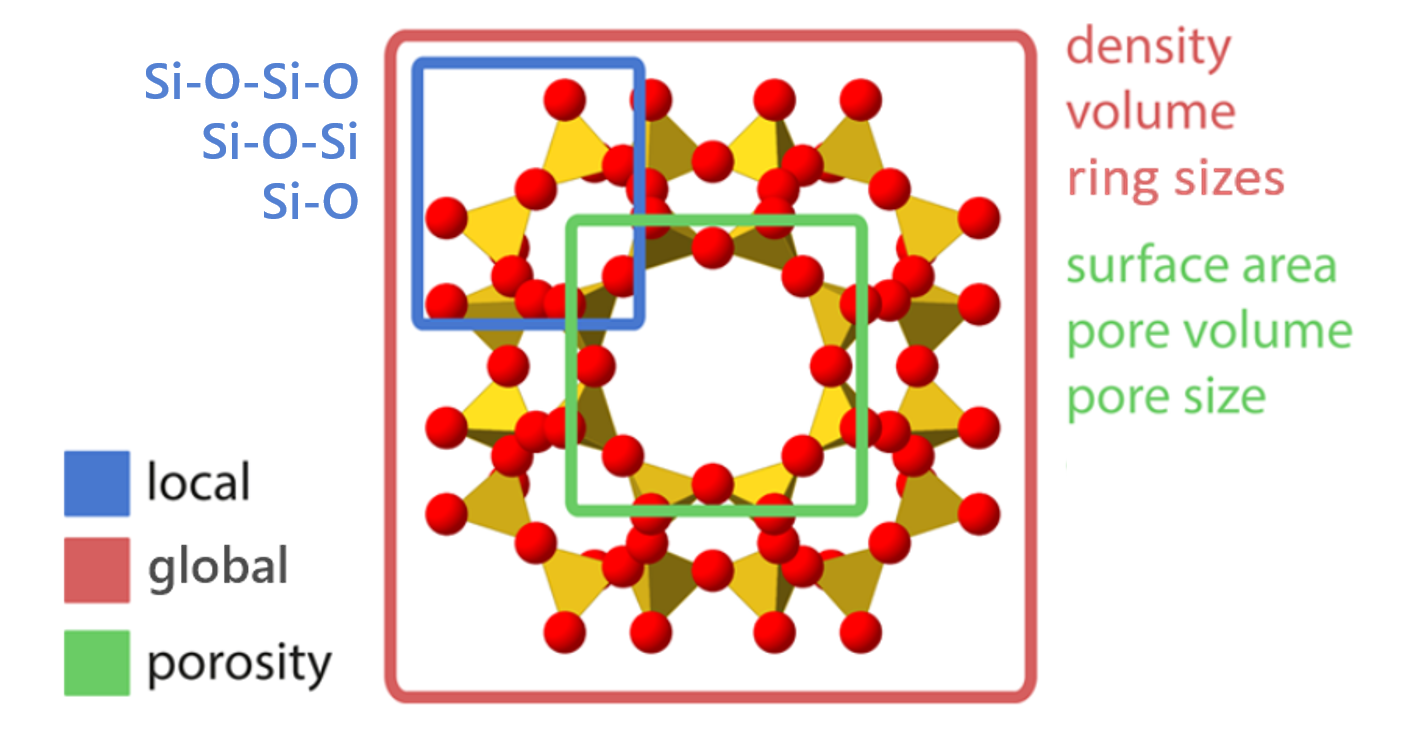
\includegraphics[clip,trim=0cm 0cm 0cm 0cm,width=0.80\textwidth]{zeolite_study_7}
\caption{Summary of the descriptors used as entries in the machine learning process classified in local properties, global properties and porosity-related properties. This figure has been taken and modified from \cite{Evans2017}.
\label{ML}}
\end{figure}

To create the predictor, we used a gradient boosting regressor (GBR)\cite{Friedman2001,Hastie2009} as implemented in Python \texttt{scikit-learn} package. This method trains regression trees as an additive model in stepwise approach by optimizing arbitrary loss functions. At each stage, a regression tree is fit on the negative gradient of the loss function. GBR is both an accurate and effective method that has been used in many areas, such as web search ranking.\cite{Mohan2011} In particular, this method was chosen over other methods such as support vector machines,\cite{Li2009} as GBR models are considered robust, interpretable, and applicable for the relatively small data set we study here.\cite{Caruana2006} The implementation of GBR employs well-established selection criteria with 3-fold cross-validation, which was repeated 100 times to give a representation of the model accuracy. The hyperparameters were chosen so as to provide good prediction accuracy and minimize overfitting. In particular, as in REF \citenum{Evans2017}, we used 1000 estimators, a learning rate of 0.01, a minimum samples split of 2, a minimum samples per leaf of 3, a maximum depth of 3, a maximum number of features equal to the square root of the number of total features and a subsample parameter of 0.4.

\begin{table}[ht]
\centering
\begin{tabular}{|c|c|}
\hline
& \textbf{descriptor}\\
\hline
\multirow{16}{*}{local}& SiO average/median/standard deviation (\AA)\\
& SiOSi average/median/standard deviation (\char23)\\& SiOSiO average/median/standard deviation (\char23)\\& SiO geometric mean (\AA)\\&  SiOSi geometric mean (\char23)\\& SiO harmonic mean (\AA)\\& SiOSi harmonic mean (\char23)\\& SiO skewness\\& SiOSi skewness\\& SiOSiO skewness\\& SiO maximum (\AA)\\& SiOSi maximum (\char23)\\& SiOSiO maximum (\char23)\\& SiO minimum (\AA)\\& SiOSi minimum (\char23)\\&SiOSiO minimum (\char23)\\
\hline
\multirow{2}{*}{global} & density\\
& numbers of N-member rings (N=3-20)\\
\hline
\multirow{7}{*}{porosity} & Largest included sphere (\AA)\\& Largest free sphere (\AA)\\& Largest included free sphere (\AA)\\&  Accessible surface area (probe radius 1.2\AA, \AA$^{2}$/\AA$^{3}$)\\&Non-accessible surface area (probe radius 1.2\AA, \AA$^{2}$/\AA$^{3}$)\\& Accessible volume (\%)\\& Non-accessible volume (\%)\\
\hline
\end{tabular}
\caption{\label{descriptors} Descriptors used in this study.}
\end{table}


\subsection{Systems studied}
As stated before, we focused on the present work on the Pophale et al. \cite{vanBeest1990} database for zeolite-like materials. In this database mechanical properties of 590811 structures were computed with BKS force-field of which 134 are known zeolitc structures. Possessing the elastic tensors (expressed as a $6\times 6$ symmetric matrix of 21 independent elastic constants $C_{ij}$.\cite{Nye1985}) of all structures in the database, we first carried out a rapid analysis of the database with ELATE with a focus on the prevalence of mechanical stability and anomalous mechanical properties. ELATE is both an open source Python module (available at \url{ https://github.com/fxcoudert/elate}) for the manipulation of elastic tensors and a standalone online application (available at \url{http://progs.coudert.name/elate}) for the routine analysis of elastic tensors based on the module. It calculates: i) average mechanical properties in the 3 averaging schemes, ii) the eigenvalues of the elastic tensor (including softest and stiffest modes), iii) minima and maxima of the elastic moduli with associated axes, iv) 2D and 3D graphs of the spatial variations of all moduli. The analysis of the database with ELATE show that: i) 128563 mechanically unstable structures ($\simeq$~22\% of the database): they correspond to local minima that are very shallow and become unstable when perturbed by small strain ($\simeq$ 1\%); ii) 578 structures are completely auxetic ($\simeq$~0.1\% of the mechanically stable structures), to the end this class of materials are labelled 3C.\\
Following statistical analysis results, we conducted 578 DFT calculations with the methodology described above of the completely auxetic subset. Then, in order to have other points of comparison, to try to generalize, especially through machine learning, the links found between structural properties and auxeticity, we secondly carried out 742 DFT calculations on randomly chosen structures in the database not including auxetic materials (the set of 742 structures are called the random set). More precisely, we will focus exclusively on the structures for which we obtained a second-order elastic rensor corresponding to a mechanically stable structure. For the completely auxetic subset, we obtained 392 mechanically stable structures from 578 structures; for the random subset, the 742 second-order elastic tensors led to 599 mechanically stable structures. We also carried to the 134 known zeolite which lead to 99 stable structures.


\section{Results and discussion}

\subsection{Noticeable elastic properties correlations}

In order to explore the existing and non-existing correlation of all the database structures computed with BKS force-field, we report the noticeable mechanical properties correlations and how it is affected when looking at hypothetical structures (590677) compared to the known ones (134 structures). Figure \ref{corr_E_rho} shows a heatmap of all the structures of the database (590811) on a density/energy graph. On top of it, the known structures are highlighted in red, and a linear fit taking into account only these structures is shown. There is a clear negative correlation between energy and density, meaning that the structures get more and more thermodynamically stable as density increases. These calculations at force-field level are in line with what was already shown by DFT calculations on a set of 121 known structures presented by Coudert in 2013.\cite{Coudert2013} Furthermore, the hypothetical structures seem to follow a similar, although not as clear, trend.

\begin{figure}[ht!]\centering
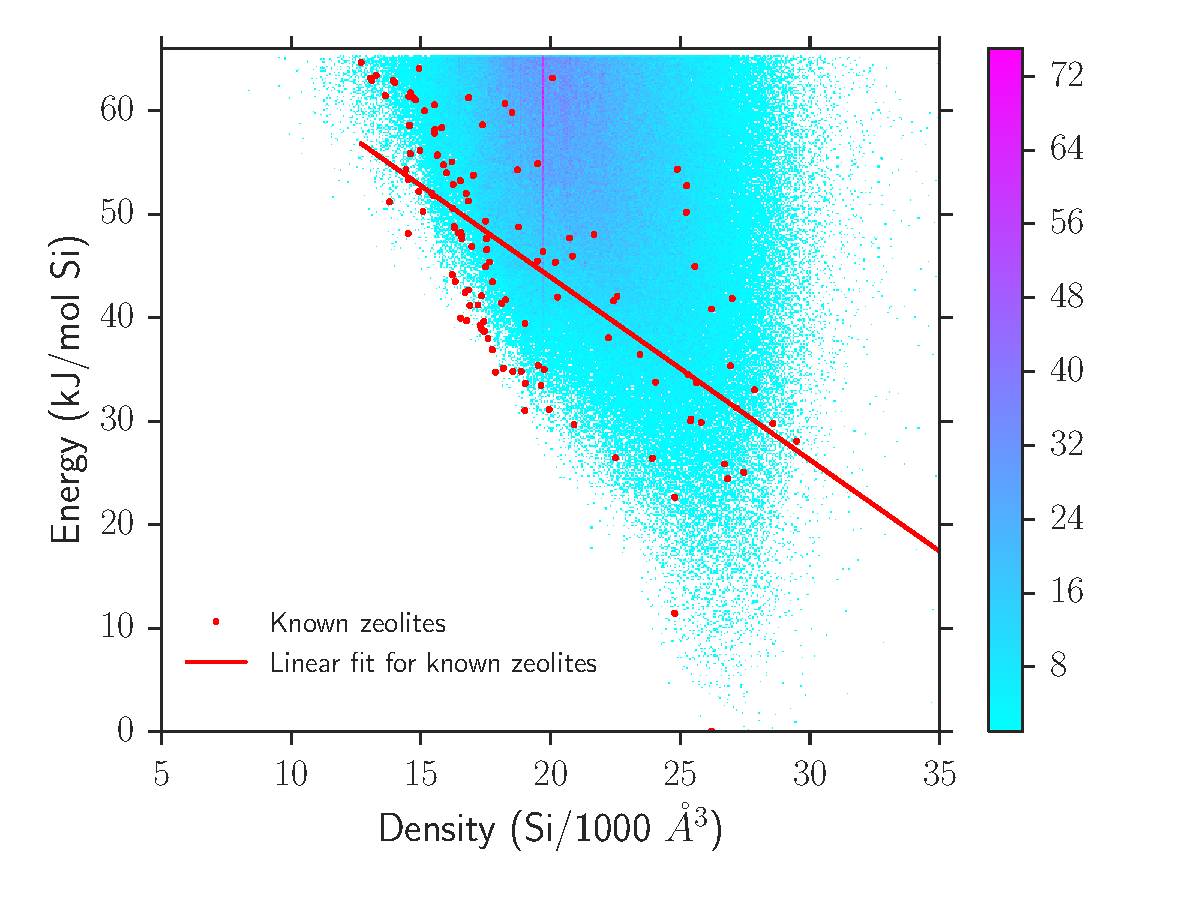
\includegraphics[clip,trim=0cm 0cm 0cm 0.8cm,width=0.8\textwidth]{deem_database_17}
\caption{Correlation heatmap between the relative energy to $\alpha$-quartz (in kJ/mol) and the density.}
\label{corr_E_rho}
\end{figure}
		
Although the force-field level calculations are able to capture the correlation between energy and density, they fail to reproduce the correlation observed on the Coudert work\cite{Coudert2013} between low elastic anisotropy (defined in Equation \ref{eq:anistropy}; directional E and G terms are determined by ELATE) and low energy. In fact, the elastic anisotropy has been proposed as a factor to determine the experimental feasibility of hypothetical structures, as very high anisotropy indicates a limited mechanical stability of the material.\cite{Coudert2013}

\begin{equation}
  \eta = \max \left( \frac{E\e{max}}{E\e{min}}, \frac{G\e{max}}{G\e{min}} \right)
\label{eq:anistropy}
\end{equation}

Figure \ref{corr_En_An} shows the correlation heatmap between elastic anisotropy and energy, with a majority of structures under 5 for the elastic anisotropy, but energy values mostly above 20 kJ/mol, whereas DFT calculations showed that an elastic anisotropy under 4 meant a very high probability of having an energy under 20 kJ/mol.\cite{Coudert2013} The preference for lower anisotropy is thus well reproduced, but the energies for known structures are overestimated. Moreover, it is important to note that low elastic anisotropy also appears to be favorable for hypothetical zeolites. In fact, most structures with energies below 30 kJ/mol have an elastic anisotropy below 5. The link is not as clear as in the case of DFT calculations for known zeolites,\cite{Coudert2013} but at least it means that having a high elastic anisotropy means being thermodynamically barely stable.

\begin{figure}[ht!]\centering
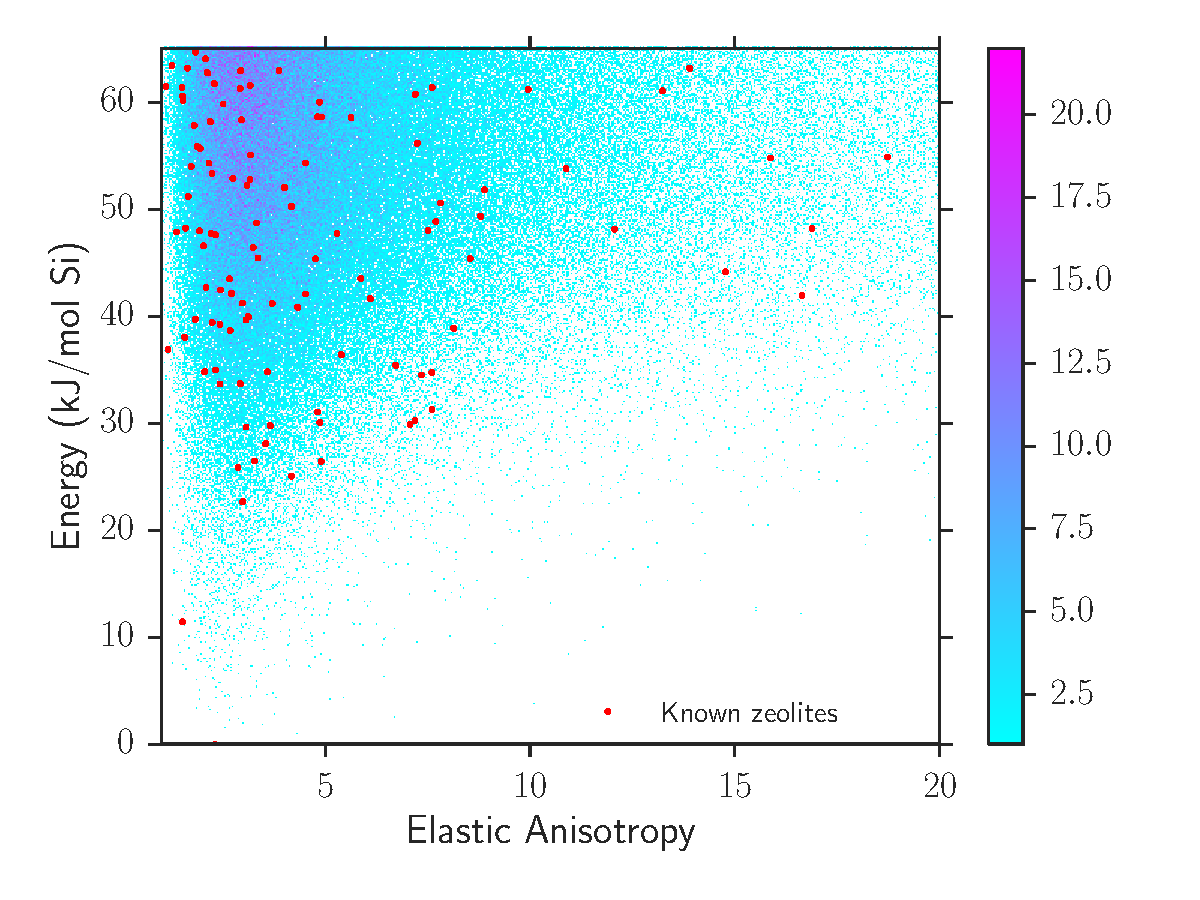
\includegraphics[clip,trim=0cm 0cm 0cm 0.8cm,width=0.8\textwidth]{deem_database_18}
\caption{Correlation heatmap between the elastic anisotropy (unitless) and the relative energy to $\alpha$-quartz (in kJ/mol).
\label{corr_En_An}}
\end{figure}
		
As mechanical anisotropy has consequences on the macroscopic behavior and stability of materials.\cite{Tan2010, Varughese2013}. In this vein, a remarkable positive correlation between minimum shear modulus and minimum Young's modulus for known zeolites is pointed out in REF \citenum{Coudert2013}. The same behavior is well captured with force-field calculations (see right panel of Figure \ref{corr_G_E}), as known structures all lie along a straight line in this $G$\e{min}-$E$\e{min} diagram. At this stage, we can say that this behaviour seems to be a generic property of any zeolitic structure as the global heatmap follows the trends for known zeolites with similar deviations. Furthermore, the left panel of Figure \ref{corr_G_E} shows that this correlation is even clearer when looking at the average values of shear and Young's moduli. It means that the basic SiO\e{4} tetrahedral unit creates a strong coupling between the response to longitudinal or shear stress, no matter the way it is assembled to form a crystal structure. The present finding reinforces the conclusions drawn earlier (ref.~\citenum{Coudert2013}) on a much larger database of zeolitic structures.
		
\begin{figure}[ht!]\centering
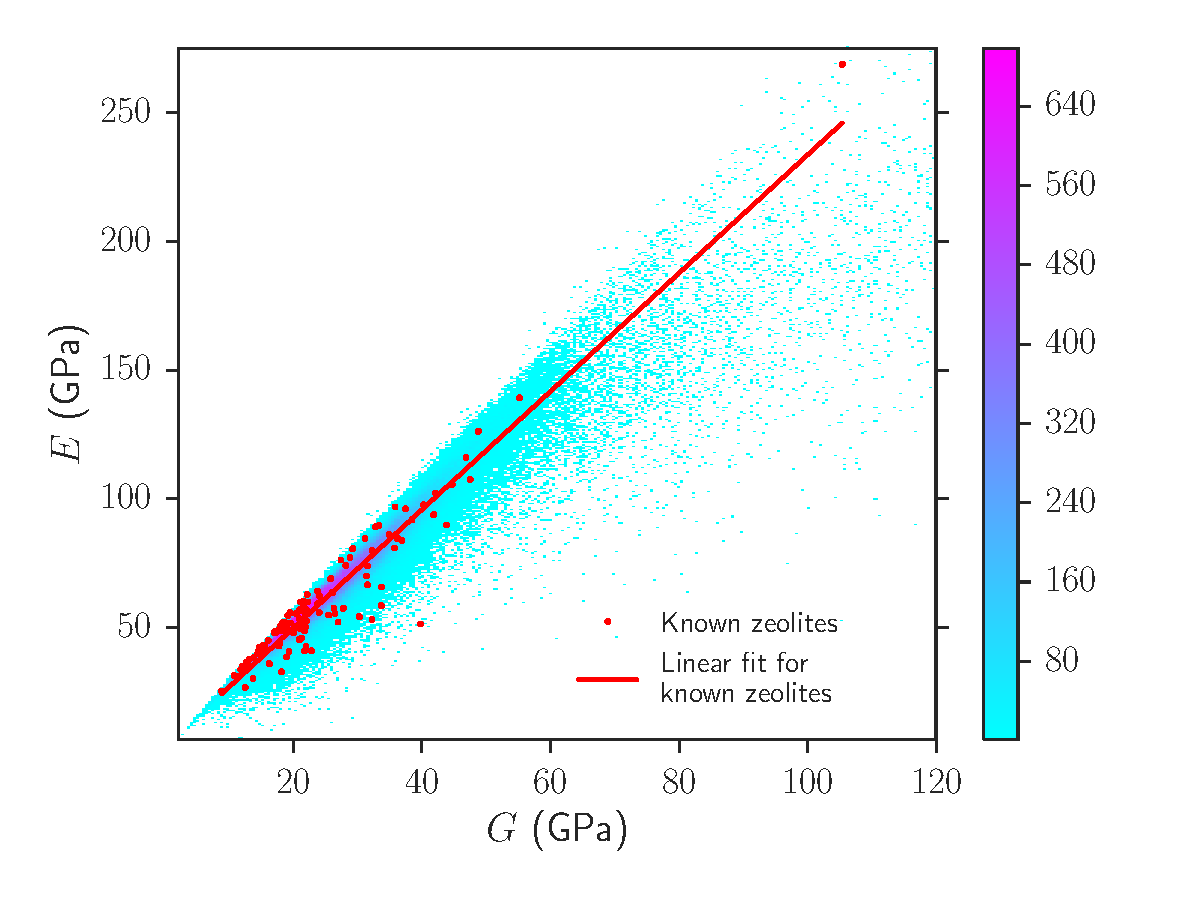
\includegraphics[clip,trim=0.7cm 0.7cm 1.3cm 0.7cm,width=0.49\textwidth]{deem_database_19_1}
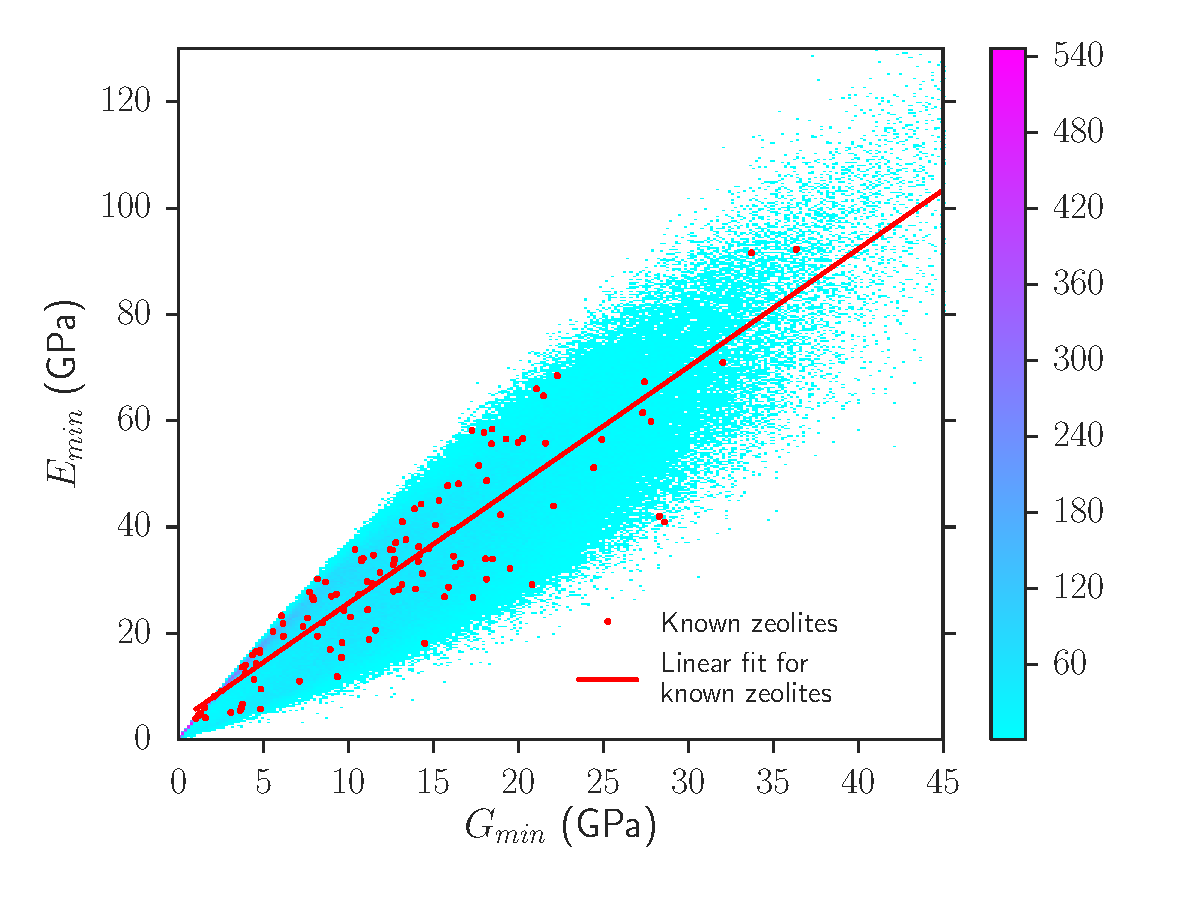
\includegraphics[clip,trim=0.5cm 0.7cm 1.5cm 0.7cm,width=0.49\textwidth]{deem_database_19_2}
\caption{Correlation heatmap between the average shear modulus $G$ (GPa) and the average Young's modulus $E$ (GPa) (left). Correlation heatmap between the minimum shear modulus $G$\e{min} (GPa) and the minimum Young's modulus $E$\e{min} (GPa) (right).
\label{corr_G_E}}
\end{figure}
If we go back to the 578 auxetic subset presented on Pophale database, in the supporting information, we show a zoom of Figure \ref{corr_G_E} with the structures of this subset highlighted with green color. The positive correlation between shear and Young's moduli seems clear for this subset too, but with lower Young's moduli overall. Another interesting feature of this subset is its average relative energy, which is very close to the one for all the zeolites, only 3 kJ/mol higher than the average for known structures. These first characteristics tend to suggest that the structures in this subset should be, for some at least, experimentally feasible.
		
Finally, we turn our attention to the correlation between extreme values of the Poisson's ratio and elastic anisotropy. It was shown that known zeolites (according to DFT calculations) behave similarly to dense silica crystals in terms of minimum and maximum Poisson's ratios following two separate families of curves when plotted agains Ledbetter anisotropy.\cite{Siddorn2015} Ledbetter anistropy is defined as the square of the maximum shear-sound-wave velocity divided by the square of the minimum shear-sound-wave velocity and characterizes mechanical anisotropy, as well as the elastic anisotropy. In Figure \ref{corr_An_Nu}, we plotted the minimum and maximum Poisson's ratios for all the zeolites, highlighting the known structures. The behaviour seen before is well reproduced for known zeolites and it can apparently be generalized for hypothetical structures as the known structures are widely dispersed among all the structures.
		
\begin{figure}[H]\centering
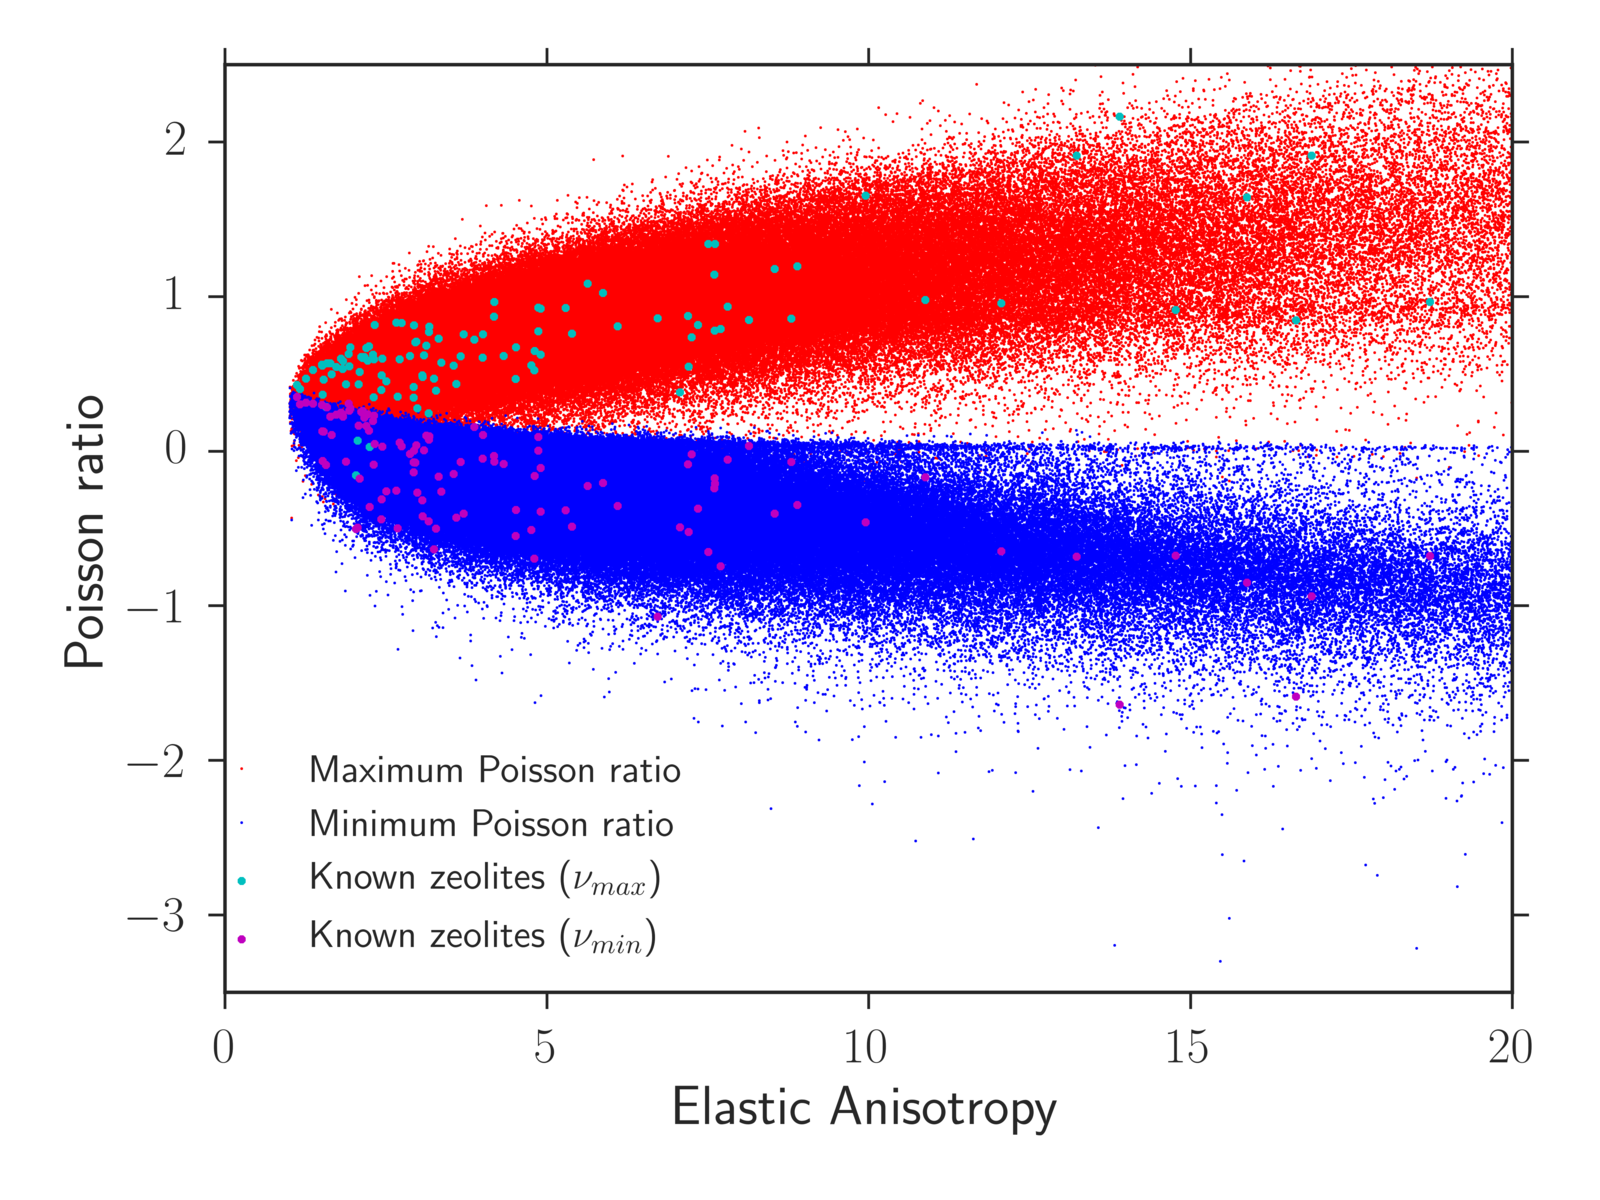
\includegraphics[clip,trim=0cm 0.25cm 0cm 0.15cm,width=0.75\textwidth]{deem_database_20}
\caption{Correlation between the elastic anisotropy and the minimum and maximum Poisson's ratios (both are unitless).
\label{corr_An_Nu}}
\end{figure}
		


\subsection{Force-field versus DFT on structural and mechanical properties}

The very large zeolitic structural Pophale database computed with BKS force-field has captured quite accurately different noticeable correlation of mechanical and energetic properties. For this reason, in this part we are interested to compare between force-field and DFT results (more computationally expensive) for the mechanically stable systems: 392 and 599 structures for the completely auxetic and random subsets, respectively. 

\subsubsection{Structural properties}

As exemplified in Figure \ref{corr_A} with the first cell parameter (a) and the angle between the second and third unit cell vectors  ($\alpha$), the cell parameters computed at the force-field level are statistically in agreement with the ones computed by DFT-D2, although there are some outliers, such as zeolite number 9316681 (numbered in the database from Pophale et al \cite{Pophale2011}) for which BKS predicted $a = 12.4$\,{\AA} and DFT gives $a = 15.8$\,{\AA}, i.e. an increase of 27\%. The volumes are also almost unchanged between DFT and force-field calculations. Furthermore these observations are independent from the subset considered, the force-field seems to perform as well on the auxetic 3C subset or the random subset.

\begin{figure}[ht!]\centering
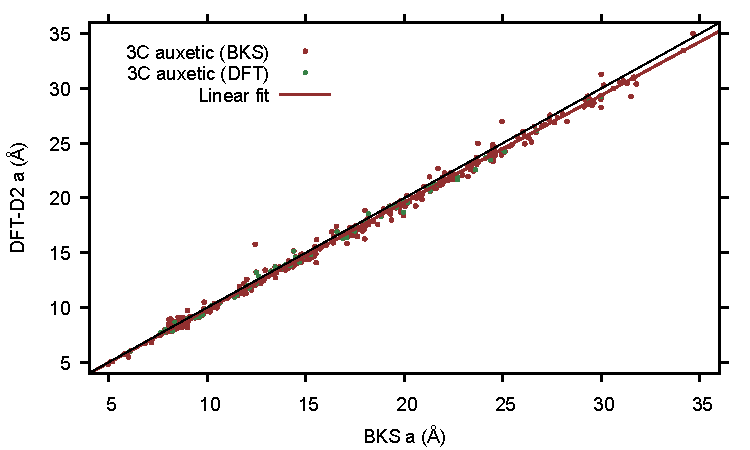
\includegraphics[clip,trim=0.05cm 0.05cm 0.25cm 0.25cm,width=0.495\textwidth]{zeolite_study_4_1}
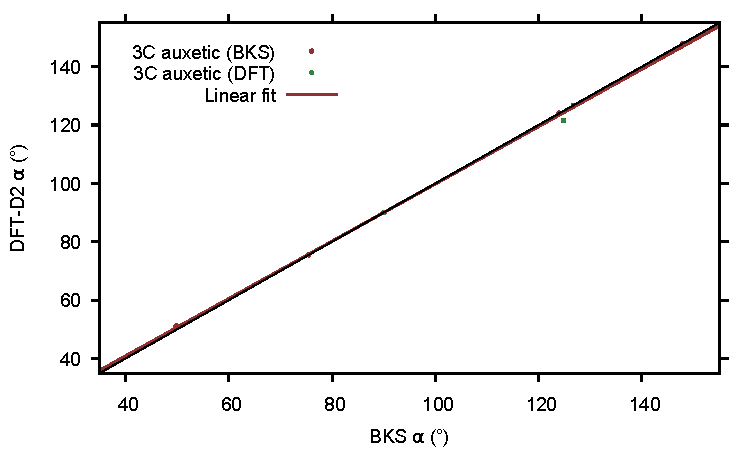
\includegraphics[clip,trim=0.05cm 0.05cm 0.25cm 0.25cm,width=0.495\textwidth]{zeolite_study_4_2}
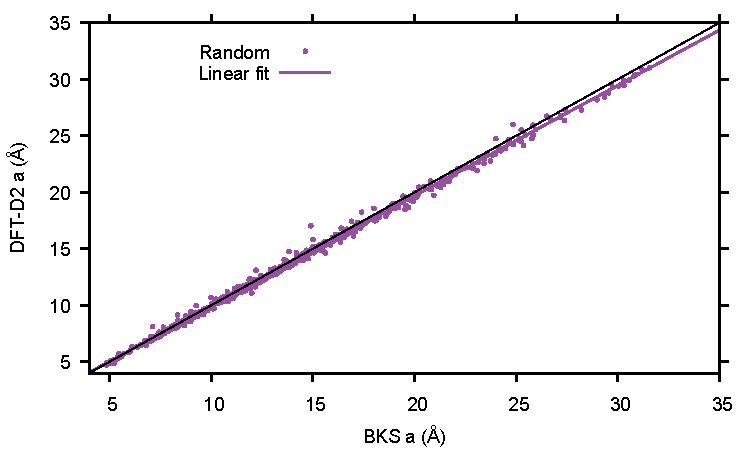
\includegraphics[clip,trim=0.05cm 0.05cm 0.25cm 0.25cm,width=0.495\textwidth]{zeolite_study_4_3}
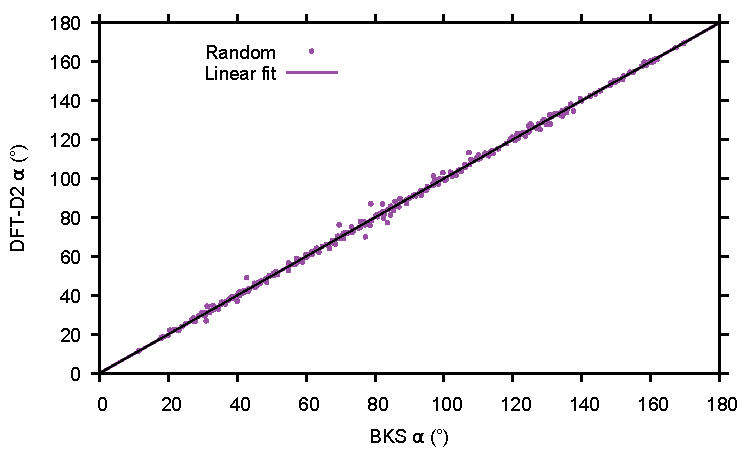
\includegraphics[clip,trim=0.05cm 0.05cm 0.25cm 0.25cm,width=0.495\textwidth]{zeolite_study_4_4}
\caption{Top panel: auxetic 3C subset, left: first cell parameter (a) given by the DFT-D2 calculations as a function of the values given by the BKS force-field. The points highlighted in green are the structures which are completely auxetic according to DFT-D2 calculations. Top panel, right: the angle between the second and third unit cell vectors ($\alpha$) given by the DFT-D2 calculations as a function of the values given by the BKS force-field. Bottom: same as top, but for the random subset. The solid black line in all graphs is the identity function.
\label{corr_A}}
\end{figure}

Although the variations for the individual cell parameters are contained, the density is more affected. As Figure \ref{corr_dens}, the agreement is still very good in average. However, on individual structures, the maximum deviation is 12\% for the random subset, but goes up to 35\% for one structure of the auxetic subset (zeolite number 9420191). The obtained results on these two sets with several hundreds of structures show that force-field based calculations of structural properties are suitable for high-throughput screening of new zeolitic structures. However, is it possible to tackle via calculations the energy and the mechanical properties, especially the Poisson's ratio with this specific force-field ? To answer this question, more details are available below. 
			
\begin{figure}[ht!]\centering
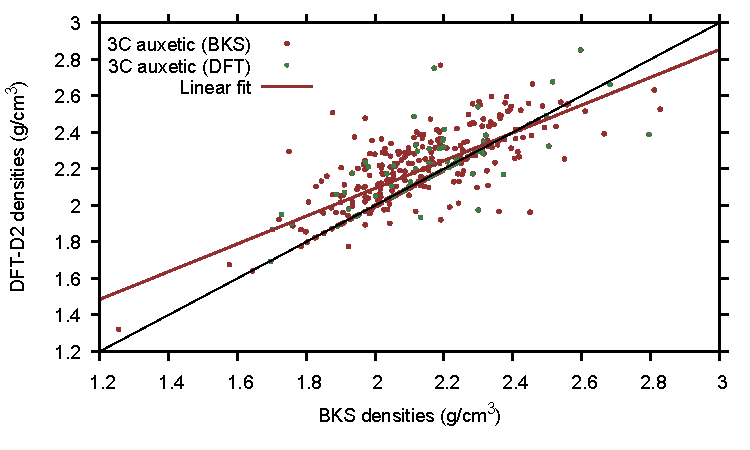
\includegraphics[clip,trim=0.09cm 0.25cm 0.25cm 0.25cm,width=0.495\textwidth]{zeolite_study_5_1}
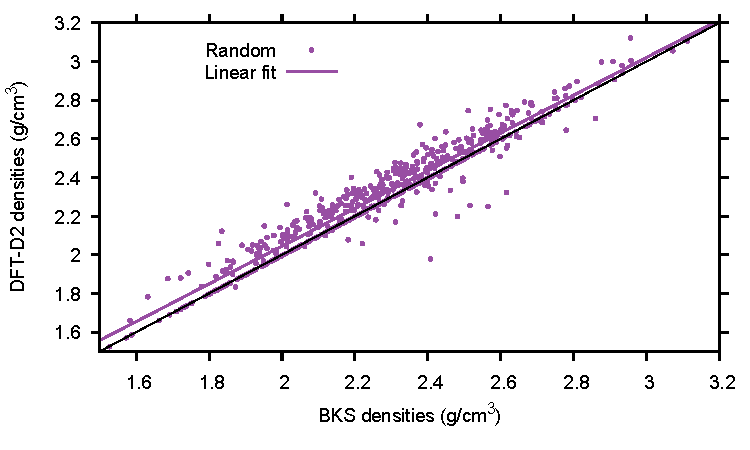
\includegraphics[clip,trim=0.09cm 0.25cm 0.25cm 0.25cm,width=0.495\textwidth]{zeolite_study_5_2}
\caption{Left: density given by the DFT-D2 calculations as a function of the values given by the BKS force-field for the auxetic 3C subset. The points highlighted in green are the structures which are completely auxetic according to DFT-D2 calculations. Right: same as left, but for the random subset. The solid black line in all graphs is the identity function.
\label{corr_dens}}
\end{figure}

			
\subsubsection{Energy and mechanical properties}
			
Figure \ref{corr_En} shows the energies given by the DFT calculations along with the ones given by the force-field level calculations. Whether it is for the auxetic subset or for the random subset, the results provided at the force-field level are completely off the DFT values. Beyond the graphical representation, the root mean square error and the mean absolute error are both above 26\,kJ/mol for both subsets. Even worse is the fact that there is rather weak correlation between the relative energies given by BKS and the ones obtained by DFT (r=0.46 for the auxetic subset and r=0.38 for the random subset).
			
\begin{figure}[ht!]\centering
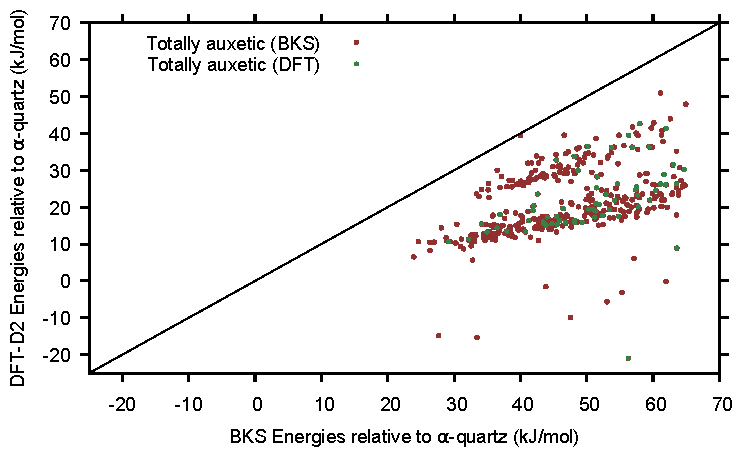
\includegraphics[clip,trim=0.15cm 0.05cm 0.25cm 0.1cm,width=0.45\textwidth]{zeolite_study_6_1}
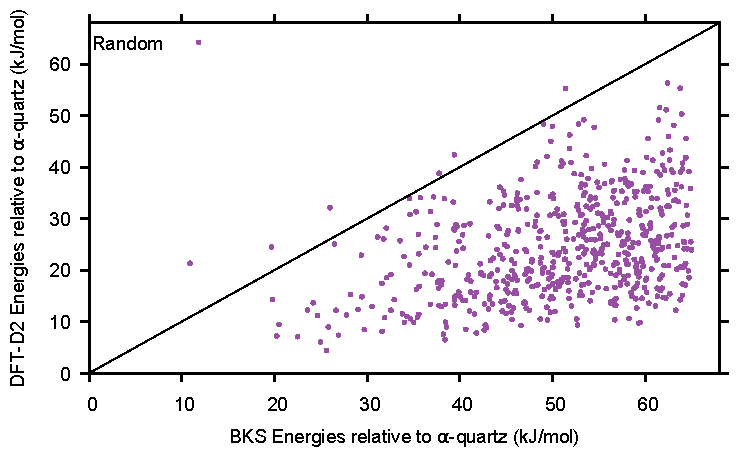
\includegraphics[clip,trim=0.15cm 0.05cm 0.25cm 0.1cm,width=0.45\textwidth]{zeolite_study_6_2}
\caption{Left: energy given by the DFT-D2 calculations as a function of the values given by the BKS force-field for the auxetic 3C subset. The points highlighted in green are the structures which are completely auxetic according to DFT-D2 calculations. Right: same as left, but for the random subset. The solid black line in all graphs is the identity function.
\label{corr_En}}
\end{figure}
			
As the second-elastic tensor coefficients depend on the variations of the energy as the material is deformed, the performance of the force-field is also quite weak on the mechanical properties. Table \ref{tab_meca_ff} shows three estimators of the deviations between DFT values and force-field values. Even taking a quite lenient measure, the relative root mean square error, which is the root mean square error divided by the range of the property in the subset considered, the lowest value is attained for the bulk modulus around 20\%. However, even in this case, the mean absolute error for the auxetic subset is 7.9\,GPa which represents almost half of the average value of the DFT bulk modulus for the auxetic subset (16\,GPa) and more than the standard deviation over this subset of 392 structures (6.5\,GPa).
			
\begin{table}[ht]
\small
\centering
\begin{tabular}{|c|c|c|c|c|c|c|c|}
\hline
 &En (kJ/mol) & $K$ (GPa)&$E$ (GPa)&$G$ (GPa)&$\nu$&$\nu_{\min}$ & $\nu_{\max}$\\
\hline
rRMSE(3C)         & 39\%          & 22\%         & 19\%        & 174\%      & 47\% & 1.93         & 1.5 \\
rRMSE(random)& 55\%          & 21\%         & 85\%        & 78\%        & 46\%& 1.35         & 13   \\
\hline
\hline
MAE(3C)           & 26                & 7.9            & 11             & 10             & 0.29 & 0.71            & 0.53  \\
MAE(random)  & 27                & 10             & 19             & 7.6            & 0.07 & 0.45            & 3.4 \\
\hline
\hline
r(3C)                  & 0.46            & 0.29           & 0.43           & -0.01        & 0.002 & 0.07            & 0.04  \\
r(random)         & 0.38            & 0.60           & 0.25           & 0.22         & 0.21& 0.03            & 0.09  \\
\hline
\end{tabular}
\caption{\label{tab_meca_ff} Relative root mean square error (rRMSE, RMSE divided by the range of the property considered), the mean absolute error (MAE) and the Pearson's correlation coefficient (r) for the energy (En), the bulk modulus ($K$), the Young's modulus ($E$), the shear modulus ($G$), the Poisson's ratio ($\nu$) and the minimum and maximum of the Poisson's ratio ($\nu_{\min}$ and $\nu_{\max}$) for auxetic and random subsets.}
\end{table}

The extreme values of the Poisson's ratio $\nu_{\min}$ and $\nu_{\max}$ are crucial in order to determine whether a material has some degree of auxeticity. Table \ref{tab_meca_ff} shows how unreliable the force-field data are in that regard. In fact, the correlation between the force-field and the DFT values is nonexistent and the very large values for the RMSE show that outliers are very badly described. The large values of the mean absolute error also shows that the force-field is unable to be accurate even for ``average'' materials. Due to the obtained results, we turned to the machine learning techniques, with the generated DFT data as training and test sets, to improve the prediction of auxeticity in these zeolitic structures.

\subsection{Predicting auxeticity}

As we have shown before, in the case of zeolite, computing mechanical properties, and in particular the Poisson's ratio is either costly (DFT) or faster but unreliable (force-field). Hence the need for more reliable and/or less costly prediction methods. In the present work,  we have appealed to machine learning in order to predict the value of Poisson's ratio for any zeolitic structure. The results are graphically represented in Figure \ref{GBR_BKS_DFT_nu}. Globally, the results given by the GBR predictor are much better than the ones given by force-field calculations. If we take the RMSE as a measure of the accuracy, it is 0.29 in the case of BKS, while it goes down to 0.12 for the GBR predictor. It is also interesting to look at the performance of the two methods on each set, the auxetic, the random and the known subsets. Table \ref{nu_gbr} gives the detail of the errors for the two models. The force-field is almost as good as the GBR predictor for the known structures. However, for hypothetical structures, and especially for the auxetic subset, the GBR predictor is at least twice as good as the force-field.
			
\begin{table}[ht]
\centering
\begin{tabular}{|c|c|c|}
\hline
Subset (method) & RMSE & MAE\\
\hline
all(GBR)  & 0.12 & 0.096      \\
all(BKS)& 0.29 & 0.15   \\
\hline
auxetic(GBR)  & 0.15  & 0.12     \\
auxetic(BKS)  & 0.34  & 0.29      \\
\hline
random(GBR)  & 0.10  & 0.079        \\
random(BKS)  & 0.26 & 0.070       \\
\hline
known(GBR)   & 0.15   & 0.13        \\
known(BKS)   & 0.18   & 0.12       \\
\hline
\end{tabular}
\caption{\label{nu_gbr} Root mean square error and mean absolute error for the 3 subsets and their assembly for the prediction of the Poisson's ratio.}
\end{table}
			
\begin{figure}[ht!]\centering
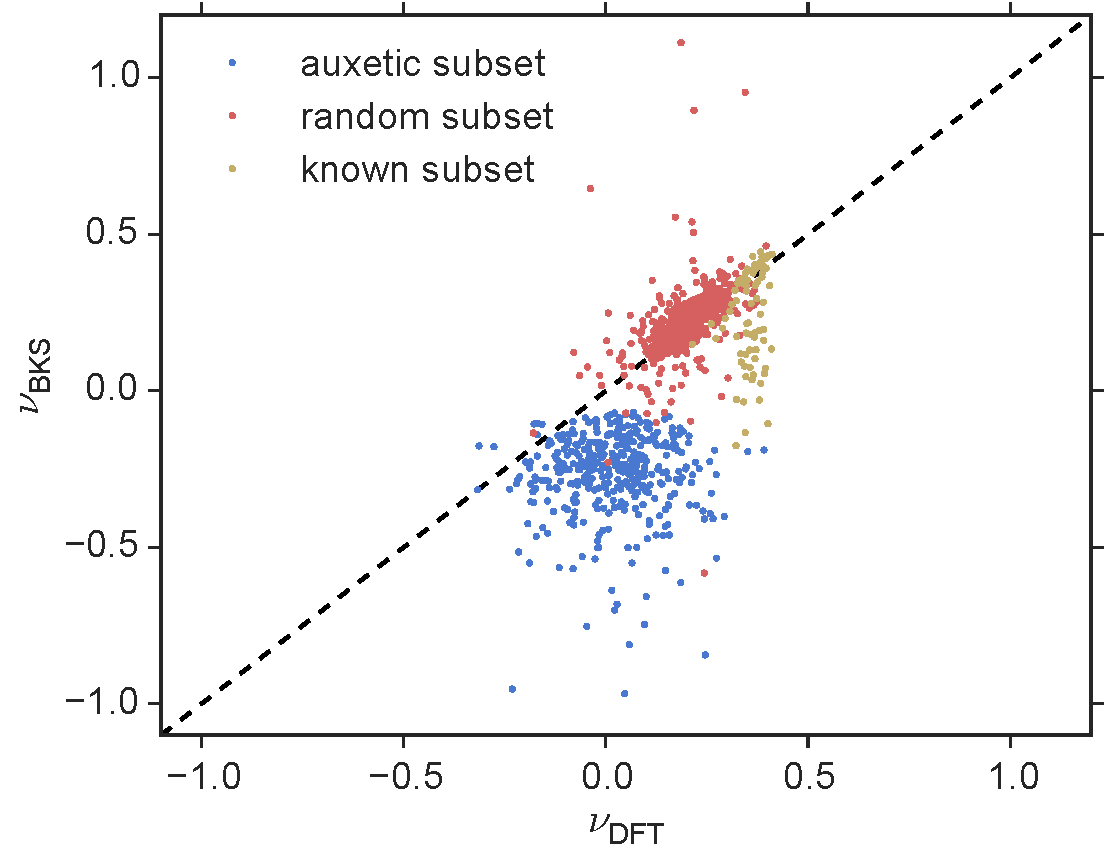
\includegraphics[clip,trim=0cm 0cm 0cm 0cm,width=0.495\textwidth]{zeolite_study_8_1}
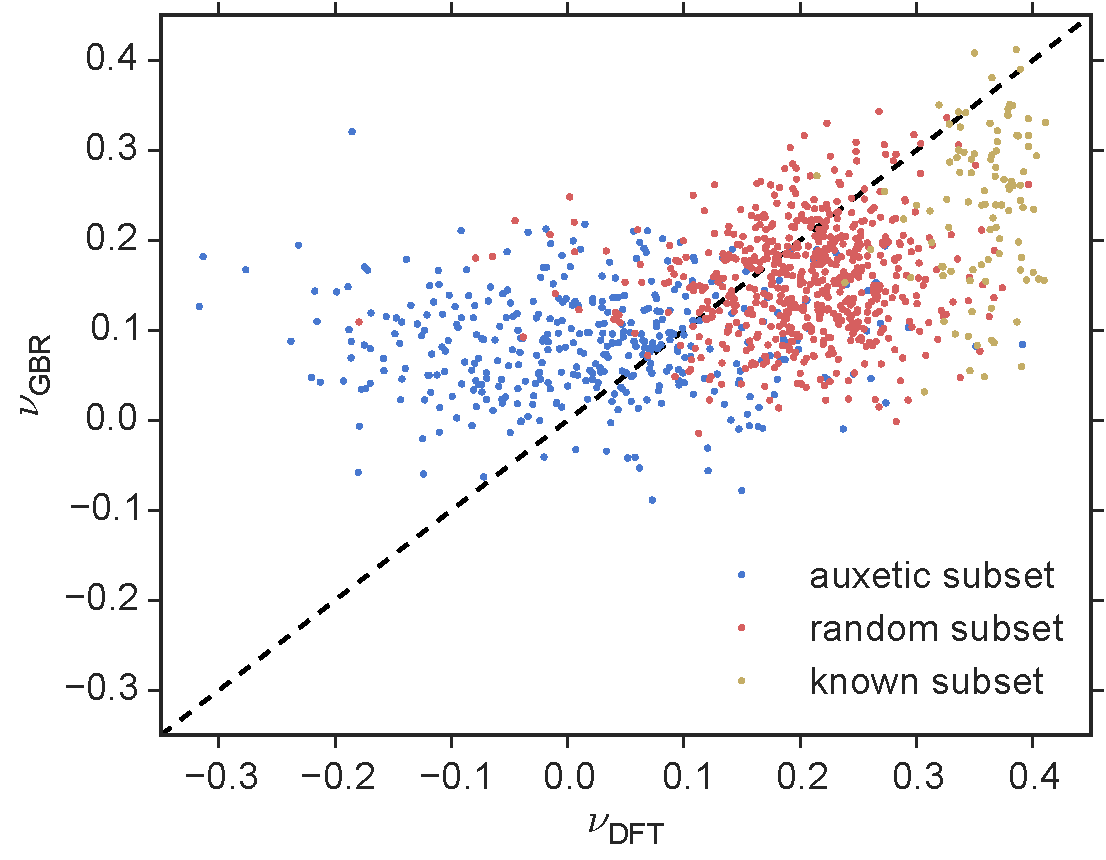
\includegraphics[clip,trim=0cm 0cm 0cm 0cm,width=0.495\textwidth]{zeolite_study_8_2}
\caption{Left: Poisson's ratio values given by BKS against values given by DFT calculations. Right: Poisson's ratio values given by GBR predictor against values given by DFT calculations. Structures from the auxetic subset are highlighted in blue, from the random subset in red and from the known subset in green.
\label{GBR_BKS_DFT_nu}}
\end{figure}
			
One of the nice feature of the GBR model is that, although it looks like a black box model, it gives the relative importance of the different descriptors after training the algorithm. It allows to build another model with less descriptors needed. In our case, we chose to keep only the descriptors with a relative importance above 40\% (compared to the most important one). Figure \ref{GBR_import} presents the relative importance of the descriptors kept for the production runs. It is interesting to see that local descriptors, and especially the amplitudes of their variations are most represented with 8 descriptors over 16. In terms of porosity-related descriptors, the linear sizes and the relative surface areas matter more than the actual porous volumes. In the global descriptors, the topology seem to play a big role with very specific ring sizes which have similar importance, namely the proportion of 4, 5, 6 and 8-member rings.
			
\begin{figure}[ht!]\centering
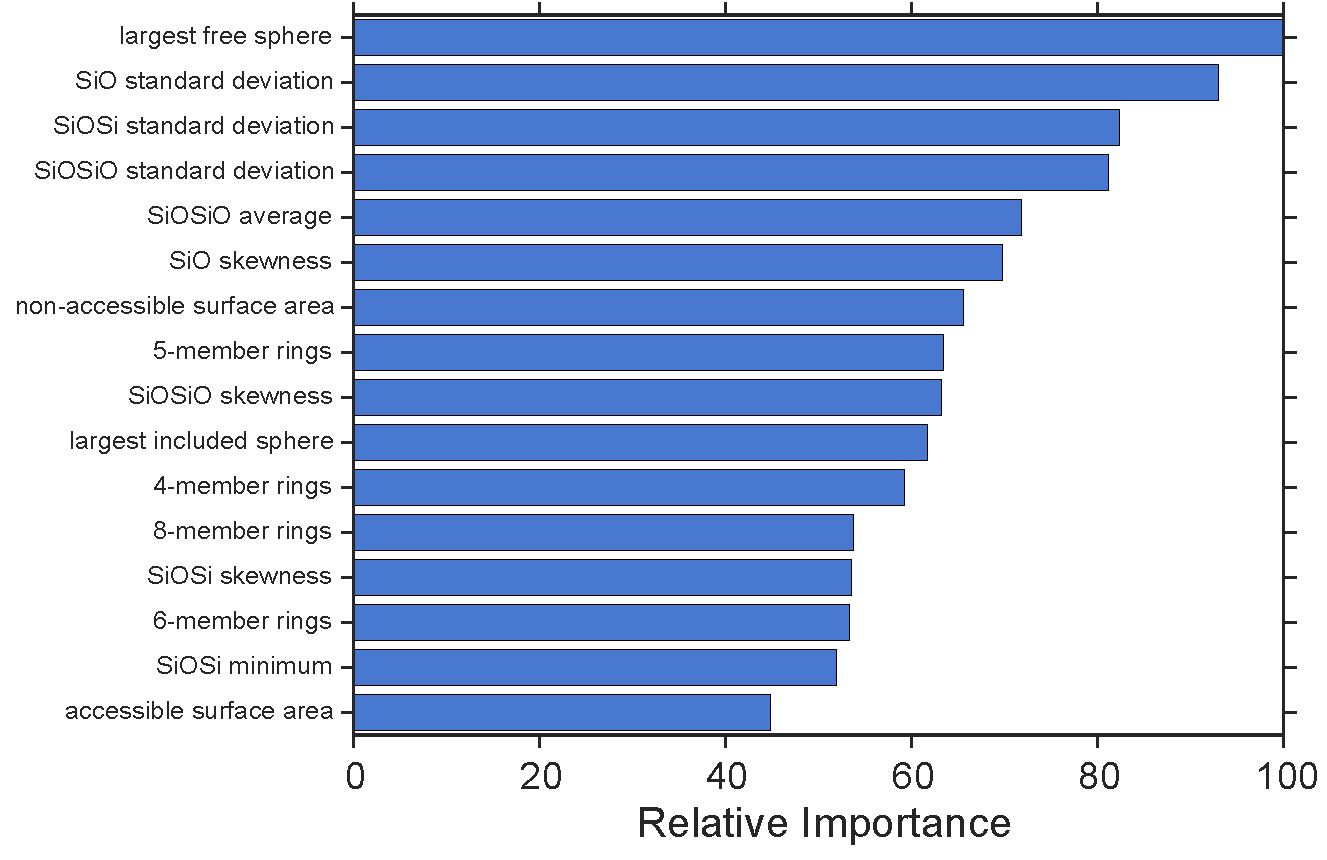
\includegraphics[clip,trim=0cm 0cm 0cm 0cm,width=0.8\textwidth]{zeolite_study_9}
\caption{Relative importance of the different descriptors actually used for production.
\label{GBR_import}}
\end{figure}
			
As the extreme values of the Poisson's ratio were particularly badly predicted (Table \ref{tab_meca_ff}) by the force-field, we conducted the exact same process for the maximum and minimum Poisson's ratio, to see if the GBR algorithm was able to create a better predictor. It turns out to be the case. Although the errors are still important, as depicted in Table \ref{numax_gbr}, they are lower than the ones obtained with the BKS force-field. In particular, looking at the errors for all the structures, the GBR model provides errors below 0.5, even for the RMSE which emphasizes the extreme cases. Looking at the errors given by the force-field, we see, again, that it cannot be used to determine auxeticity. Although my models are not perfect they give a promising way of having low-cost models to predict auxeticity in zeolites.
			
\begin{table}[ht!]
\centering
\begin{tabular}{|c|c|c|c|c|}
\hline
Subset (method) & RMSE($\nu_{\min}$) & MAE($\nu_{\min}$) & RMSE($\nu_{\max}$) & MAE($\nu_{\max}$)\\
\hline
all(GBR)  & 0.39 & 0.26 & 0.46 & 0.32      \\
all(BKS)& 1.4 & 0.51 & 9.8 & 2.1  \\
\hline
auxetic(GBR)  & 0.38  & 0.25   & 0.46 & 0.34  \\
auxetic(BKS)  & 1. 5 & 0.66  & 0.62 & 0.47    \\
\hline
random(GBR)  & 0.40  & 0.25    & 0.48 & 0.31    \\
random(BKS)  & 1.4 & 0.45    & 13 & 3.4   \\
\hline
known(GBR)   & 0.43   & 0.35   & 0.34 & 0.27     \\
known(BKS)   & 0.50  & 0.35   & 0.47 & 0.32    \\
\hline
\end{tabular}
\caption{\label{numax_gbr} Root mean square error and mean absolute error for the 3 subsets and their assembly for the prediction of the Poisson's ratio.}
\end{table}

\section{Conclusions and perspectives}

Using quantum chemistry calculations at the DFT level on two large sets extracted from a structural database of about 600,000 hypothetical zeolitic structures, we were able to show that the BKS force-field can be used to reliably predict structural properties of hypothetical all-silica zeolites. However, concerning mechanical properties, especially the Poisson's ratio, and even more precisely its extreme values, this force-field is unusable for screening potentially auxetic materials. Then, we have shown that machine learning techniques offer a way to build fast and more reliable predictive models, as we did for the Poisson's ratio and its extreme values. The only issue with these types of methods is their ``black-box'' behaviour. Nonetheless, most of them are still able to attribute relative importance to the descriptors they are given. Finally, the present finding focuses on all-silica zeolites, but it could absolutely be applied to all sorts of porous materials, given a large enough reliable database based on experiments or quantum calculations.


\begin{acknowledgement}
We acknowledge access to high-performance computing platforms provided by GENCI grant A0050807069.
\end{acknowledgement}

\begin{suppinfo}



\end{suppinfo}

\bibliography{achemso-demo}

\end{document}